\documentclass[UTF8]{ctexart}
\hfuzz=4pt

\usepackage{parskip}
    \setlength{\parindent}{0em}
    \setlength{\parskip}{1em}
\usepackage{geometry}
    \geometry{left=4cm,right=4cm,top=2cm,bottom=2cm}
\usepackage{amsmath, amssymb, amsthm, mathtools}
\usepackage{thmtools}
    \renewcommand\qedsymbol{$\blacksquare$}
    \declaretheorem[numberwithin=section,shaded={rulecolor=cyan,rulewidth=2pt,bgcolor=white}]{definition}
    \declaretheorem[numberwithin=section,shaded={rulecolor=orange,rulewidth=2pt, bgcolor=white}]{theorem}
    \newtheoremstyle{mystyle}{1em plus .2 em minus .2em}{1em plus .2 em minus .2em}{}{}{\bfseries}{.}{.5em}{}
    \theoremstyle{mystyle}
    \newtheorem{axiom}{Axiom}[section]
    \newtheorem{lemma}{Lemma}[section]
    \newtheorem{proposition}{Proposition}[section]
    \newtheoremstyle{myremark}{1em plus .2 em minus .2em}{1em plus .2 em minus .2em}{}{}{\itshape}{.}{.5em}{}
    \theoremstyle{myremark}
    \newtheorem*{remark}{Remark}
    \theoremstyle{plain}
    \newtheorem{corollary}{Corollary}[section]
\usepackage{caption}
\usepackage{xcolor}
\usepackage{graphicx}
\usepackage{float}
\usepackage{setspace} 	 % 行间距 \begin{spacing}{arg}
\usepackage{esint}
\usepackage{hyperref}
    \hypersetup{colorlinks=true,linktoc=all,linkcolor=blue}

\newcommand{\ve}[1]{\boldsymbol{\mathbf{#1}}}
\newcommand{\unit}[1]{\boldsymbol{\mathbf{\hat{#1}}}}
\renewcommand{\r}{\mathrm}
\renewcommand{\cal}{\mathcal}
\newcommand{\scr}{\mathscr}

\newcommand{\E}{\mathrm e}
\renewcommand{\I}{\mathrm i}
\newcommand{\R}{\mathbb R}
\newcommand{\Z}{\mathbb Z}
\newcommand{\N}{\mathbb N}
\newcommand{\Q}{\mathbb Q}
\renewcommand{\C}{\mathbb C}
\DeclarePairedDelimiter\set{\{}{\}}
\newcommand{\del}{\nabla}

\pagestyle{empty}

\begin{document}
\section{图与子图}

图有两种定义方式, 一个为二元组, 一个为三元组.

\begin{definition}[\text{图}]
    图 $ G $ 为一个三元组 $ G \coloneqq (V, E, \psi) $, $ V $ 为顶点的集合, $ E $ 为边的集合, $ \psi $ 为边和顶点对的对应关系. 若隐式地的定义边和顶点对的对应关系, 则可以定义 $ G \coloneqq (V, E) $. 对于给定的图 $ G $, 可以记 $ V(G) $, $ E(G) $ 分别代表 $ G $ 的顶点和边集.
\end{definition}

\begin{figure}[H]
    \centering
    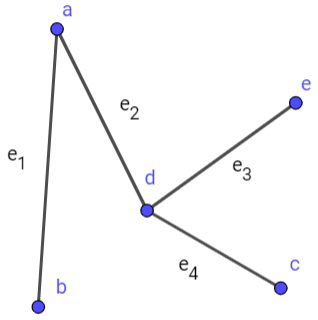
\includegraphics[width = 0.35\linewidth]{./images/graph_definition.png}
    \caption{图 $ G = (V, E, \psi) $}
\end{figure}

\paragraph{例}
上图 $ G $, 其顶点集 $ V = \set{a, b, c, d, e} $, 边集 $ E = \set{e_1, e_2, e_3, e_4} $. 而边和点之间的对应关系为:
\[ \begin{array}{c}
    \psi(e_1) = (a, b) \,,\\
    \psi(e_2) = (a, d) \,,\\
    \psi(e_3) = (d, e) \,,\\
    \psi(e_4) = (d, c)
\end{array} \,.\]

下面概念描述了由原图得到其它图.
\begin{definition}[\text{子图}]
    设图 $ G = (V, E) $, $ V' \subseteq V $, $ E' \subseteq E $, 则图 $ G' = (V', E') $ 称为 $ G $ 的子图. 若 $ G' \neq G $, 则称 $ G' $ 为 $ G $ 的真子图.
\end{definition}

相比子图, 导出子图的概念更常见.

\begin{definition}[\text{点导出子图}]
    设 $ G = (V, E) $, $ V' \subseteq V $. 定义 $ V' $ 的点导出子图 (vertex-induced subgraph) 为 $ G(V') = (V', E') $, 其中:
    \[ E' \coloneqq \set{(a, b) \in E \mid a, b \in V'} \,.\]
\end{definition}

换句话说, $ G(V') $ 的边集由 $ E $ 中关联 $ V' $ 中任意顶点的的边构成. 这意味着两方面: (1) $ V' $ 中任意两点若在 $ G $ 中关联, 则这条边就在导出子图中; (2) 若 $ (a, b) $ 为导出子图中的一条边, 则 $ a, b $ 在原图中也是关联的.

同理还可得到边导出子图.

\begin{definition}[\text{删除点}]
    对于图 $ G = (V, E) $, 设 $ v \in V $. 则删掉这个点及其关联的边, 剩下的图记作 $ G - v $. 也即:
    \[ \begin{cases}
        V(G - v) \coloneqq V - \set{v} \\
        E(G - v) \coloneqq \set{(a, b) \in E \mid a \neq v \land b \neq v} 
    \end{cases} \,.\]

    注意: $ E(G - v) $ 的等价定义为 $ \set{(a, b) \in E \mid a, b \in V - \set{v}} $.
    \vskip 1em
    同理还可以得到删除多个点及其中每个点关联的边得到的图, 记点集 $ V' \subseteq V $. 则 $ G - V' $ 可以定义为:
    \[ \begin{cases}
        V(G - V') \coloneqq V - V' \\
        E(G - V') \coloneqq \set{(a, b) \in E \mid a, b \in V - V'} 
    \end{cases} \,.\]
\end{definition}

从导出子图以及删点子图的定义, 不难得到下面的结论:
\begin{proposition}
    设 $ G = (V, E) $, 若 $ V' $ 和 $ V'' $ 为 $ V $ 的一个划分, 即: $ V' \cap V'' = \varnothing $ 且 $ V' \cup V'' = V $. 则有:
    \[ G(V') = V - V'' \,,\]
    \[ G(V'') = V - V' \,.\]
\end{proposition}

也就是说, 导出子图 $ G(V') $ 可以定义为删去所有除 $ V' $ 之外的点 (即 $ V'' $) 以及其关联的边后剩下的图.


\section{连通性}
\begin{definition}[\text{道路, 简单道路与路径}]
    定义道路 (walk) 为一系列交替的点和边的序列: $ v_0, e_1, v_1, e_2, v_2, \dots, e_n, v_n $; 其中 $ e_i $ 关联 $ v_{i - 1} $ 和 $ v_i $. 
    \begin{itemize}
        \item 若道路中除首尾两个点, 没有相同的节点, 即对任意 $ 1 \leqslant i, j \leqslant n - 1 $, 有 $ v_i \neq v_j $, 则称该道路为简单道路 (path)
        \item 若道路中没有重复的边, 则称其为路径 (trail)
        \item 若道路首尾两点为同一点, 则称其为回路; 若简单道路的首位两点为同一点, 则称其为简单回路
    \end{itemize}
\end{definition}

对于道路 $ v_0, e_1, v_1, \dots, v_{n - 1}, e_n, v_n $, 其含有 $ n $ 条边, 称这条道路的长度为 $ n $, 记作 $ d(v_0, v_n) = n $.

下面几张示意图描述了上面几个术语之间的区别, 注意箭头并不表示有向图, 数字也不代表赋权, 此处只是形象化的表示出这条道路从起点到终点的行进过程和顺序.
\begin{figure}[H]
    \centering
    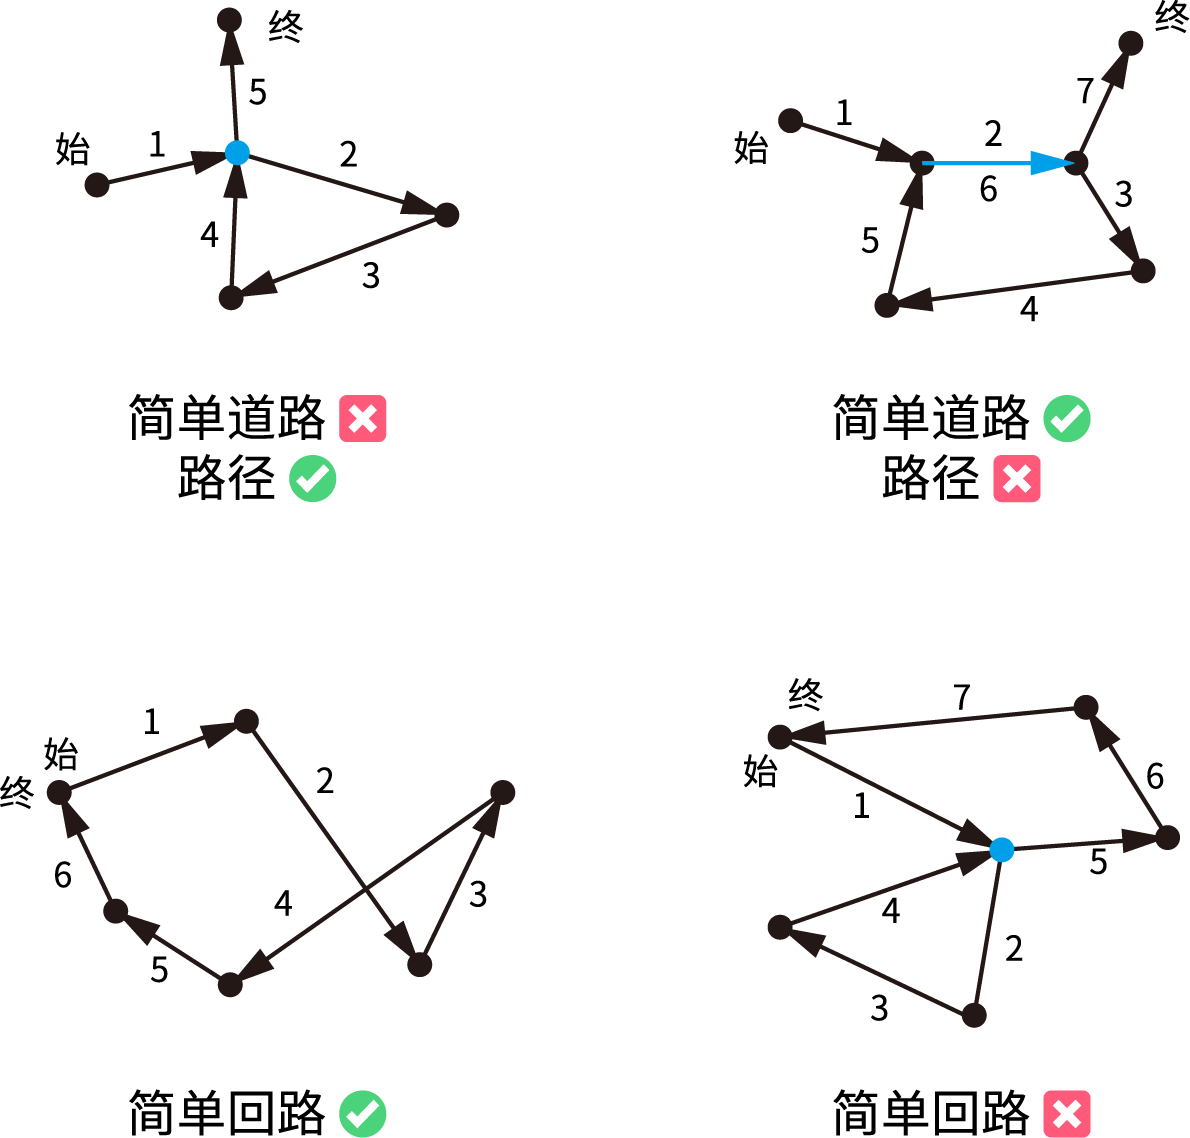
\includegraphics[width = 0.7\linewidth]{./images/path_trail.png}
\end{figure}







\end{document}